\section{Problematic Solutes in NF}

\rod{Summary of most problematic ions in CT}


\subsection{Calcium Carbonate }
\label{Calcium_carbonate_carbonatesystem_teori}

\rod{Dette afsnit er ikke helt gennem arbejdet, vi vil gerne have feedback på hvad der mangler.}

%ca carobnate scaling. 
Calcium carbonate is one of the most common scaling agents, precipitating via the breakdown of calcium bicarbonate \citep{IntroductionCoolingTower2014}. 
Calcium ions forms complexes with carbonate forming \ce{CaCO3} which has very low solubility. \citep{WaterChemistry1980}
The solubility of \ce{CaCO3} is influenced by the partial pressure of \ce{CO2}, temperature and the presence of other salts. %kilde 1929 CaCO3
%The solubility of \ce{CaCO3} decrease with increase in temperature, \citep{IntroductionCoolingTower2014} 
%and is also influenced by the partial pressure of \ce{CO2}, and presence of other salts. %kilde 1929 CaCO3
%, bicarbonate can be monitored to help control scaling.
The precipitation of calcium carbonate is therefore directly affected by the carbonate system. \citep{WaterChemistry1980}

%Calcium reacts with carbonate 
% \begin{align}
%     \cee{Ca^{2+} + HCO3- &<=> CaCO3_{(s)}} + H+ \\
% \end{align}


The carbonate system is the most important acid-base system in water. \citep{WaterChemistry1980}
%The ability of natural waters to maintain pH is due to the carbonate system which has buffer capacity in pH range 6.0-6.6 \citep{WaterChemistry1980}
The partial pressure of \ce{CO_2} in the atmosphere is in equilibrium with the carbonic acid (\ce{H2CO3}) concentration in solution. 
Carbonic acid deprotonates to produce bicarbonate or carbonate and these equilibrium reactions are what constitutes the carbonate system.\citep{WaterChemistry1980} 

\begin{align}
    \cee{CO2_{(g)} &<=> CO2_{(aq)}} \\
    \cee{CO2_{(g)} H2O &<=> H2CO3}\\ 
    \cee{H2CO3 &<=> H+ + HCO3-} \\
    \cee{HCO3- &<=> H+ + CO3^{2-}}
\end{align}

This means that increasing partial pressure of \ce{CO2} the surroundings leads to an increase in \ce{CO3^{2-}} concentration and increased risk of calcium carbonate precipitation. 
%\rod{Hvordan påvirker CO2 partial pressure solubility?}
Likewise, changes in pH also influence the presence of carbonate ions in solution, where a higher pH leads to higher fraction of carbonate ions present, see \cref{fig:pH_pC}. 


\begin{figure}[H]
    \centering
    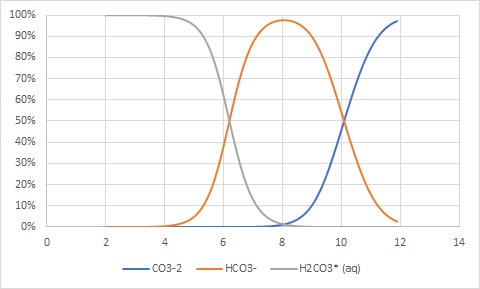
\includegraphics[width=0.7\textwidth]{Billeder/teori/pH_pC_Carbonat.png}
    \caption{pH pC Carbonate, made in MINTEQ}
    \label{fig:pH_pC}
\end{figure}


%Ph effekt på carbonat system, hvad sker der. 
Alkalinity is the capacity of water to neutralize strong acid and total alkalinity is defined as 2[\ce{CO3^{2-}}]+[\ce{HCO3-}]+[\ce{OH-}]-[\ce{H}].  \citep{WaterChemistry1980}
Alkalinity is reduced when \ce{CaCO3} precipitates as \ce{CO3^{2-}} is removed from solution. \citep{WaterChemistry1980}
Other species such as silicates also contribute to total alkalinity. \citep{WaterChemistry1980} 
Once a system has overcome hardness issues, the next scaling problem usually occurs with silica. \citep{ChemistrySilicaScale2014}

%Furthermore, if ion exchange is implemented higher sodium concentration will occur and should be monitored to investigate the charge balance.



%During a titration some of the base is converted by the conjugate acid. \citep{WaterChemistry1980}
%Naturals water capacity to neutralize strong base is due to \ce{H2CO3-} \ce{HCO3-} and \ce{H+}
%A buffer solution maintain stable composition when other components are added or removed. \citep{WaterChemistry1980}
%Solutions must be supersaturated before precipitate will form from homogeneous solution. \citep{WaterChemistry1980}
%(CaCO3 solubility constant 8.34 or 8.22 pKa)
%pH of natural waters is influenced by the carbonate system and further influence solubility of some metal ions.  

%Charge balance must be met in water samples, where the total number of positive charges must equal the equivalent negative charge. For waste waters the charge neutrality must agree within +/- 5\% and for seawater it should be within +/- 2\%, larger deviations indicate error or missing species in the analysis. \citep{WaterChemistry1980}

\subsection{Silica}
\label{Silica_teori_ladning}
\rod{Få det relateret til NF i forhold til ladning. få silica ladning i forhold til pH billede med. }



Problems regarding silica scaling are a result of the complex silica chemistry and scale formation where multiple different mechanisms can take place, and once formed the scaling is difficult to remove. \citep{ChemistrySilicaScale2014}
In solution silica exists in multiple soluble forms; monomeric, polymeric, %formed by dehydration of individual silicic acid molecules that make Si-O bond.
colloidal, %small silica particles, 5 nm or greater, non reactive.
particulate %larger than colloidal, 0.45 micro meter
and as silicate ions. 
Silica \ce{(SiO2)} is present in groundwater, due to weathering of silicate minerals, where silica hydrolyses and forms \ce{H4SiO4}, see \rod{XX}. \citep{ChemistrySilicaScale2014}
%When silica concentration is below 200 mg/L silica exists in monomeric form.
At neutral pH silicic acid \ce{H4SiO4} is the main soluble silica species, which is a weak acid that can undergo deprotonation and form ionic species according to eq \rod{XX and XX}. \citep{ChemistrySilicaScale2014}

\begin{align}
    \cee{ SiO2 + 2 H2O &<=> H4SiO4} \\
    \cee{H4SiO4 &<=> H+ + H3SiO4-}\\ 
   \cee{H4SiO4 &<=> 2H+ + H2SiO4^{2-}} 
\end{align}
%\citep{ChemistrySilicaScale2014}

%pH. %temperature. 
The solubility of silica is dependant on pH and temperature. %where scaling can take place by deposition on membrane, polymerization and accumulation of colloidal particles. \citep{ChemistrySilicaScale2014} 
% The formation ionic silica species are believed to lead to increased solubility at high pH, but also assist in precipitation of silica. 
% Silica has minimum solubility around 100  mg/L at pH 7-8, increasing rapidly around pH 9 to about 876 mg/L at pH 10.6. \textcolor{blue}{måske se billede, find rigtig kilde pt} \cite{ChemistrySilicaScale2014}
% %at pH > 8.5 silica is soluble at 250 ppm as \ce{SiO2} which drops to a solubility of 150 ppm at pH 7.5. \citep{IntroductionCoolingTower2014}
% When silicic acid concentration exceed 200 mg/L a reversible polymerization can take place, which involve both ionic and non-ionic silicic acid molecules in a condensation reaction. 
% Polymerization can lead to further aggregation and ultimately particle formation, kinetics of this polymerization is generally slow, but results indicate highest kinetics at pH 6.5-7.5 \textcolor{blue}{evt. læs direkte kilde.}. Ultimately meaning more rapid silica scaling at high pH despite increase in silica solubility. \citep{ChemistrySilicaScale2014}
Silica has minimum solubility of 100  mg/L at pH 7-8, increasing with pH starting around pH 9, and reaching ~875 mg/L at pH 10.6. 
The formation of ionic silica species is believed to lead to increased solubility at high pH. \citep{ChemistrySilicaScale2014} %but also assist in precipitation of silica. 
Where the ionic silica is present in higher fractions at higher pH, and most silica species in solution are charged at pH above 10, see \cref{fig:silica_pH_fraktion}. 

%\textcolor{blue}{måske se billede, find rigtig kilde pt} \cite{ChemistrySilicaScale2014}
%\rod{her kunne der komme noget om silica species fraction mod pH, fra minteq.}

\begin{figure}[H]
    \centering
    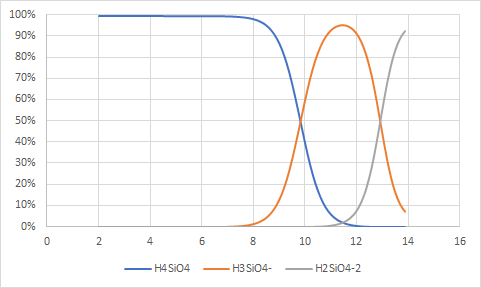
\includegraphics[width=0.7\textwidth]{Billeder/teori/pH_pC_Silica.png}
    \caption{Speciation of silicates. Calculated with MINTEQ}
    \label{fig:silica_pH_fraktion}
\end{figure}



%at pH > 8.5 silica is soluble at 250 ppm as \ce{SiO2} which drops to a solubility of 150 ppm at pH 7.5. \citep{IntroductionCoolingTower2014}
When silicic acid concentration exceeds 200 mg/L a reversible polymerization can take place, which involves both an ionic and non-ionic silicic acid monomer in a condensation reaction. 
As the polymerization reaction occurs due to the presence of ionic silica species, higher pH values can lead to further aggregation and particle formation as ionic species are present at larger fractions.
Meaning that the apparent increased solubility of silica at high pH, also can lead to polymerization and possible scaling.   \citep{ChemistrySilicaScale2014}
Silica scaling can also form in an acidic environment where two non-ionic silicic acid molecules react, but this reaction is typically slower. \citep{ChemistrySilicaScale2014}
The solubility of silica also increases with rising temperatures, but depend on the silica species present. 
Increased temperatures will also increase the kinetics of the above-mentioned polymerization causing scale formation and thus reduced solubility over short time-periods. \citep{ChemistrySilicaScale2014}
%membrane


%cations
Additionally, presence of cations can decrease apparent solubility of silica and lead to formation of insoluble metal silicates, even below silica saturation concentration. 
At pH between 6.5 and 10.5 above-mentioned polymeric silica species remain negatively charged and do not aggregate, but monovalent cations e.g. \ce{Na+} can neutralize these particles leading to aggregation of particles. 
Di- and trivalent cations e.g. \ce{Ca^{2+}} act as bridges between different particles participating in the process of aggregation. \citep{ChemistrySilicaScale2014}
%At high pH metal silicate easily form with different solubilities, where aluminium and iron has shown to often be part of silica scaling. \citep{ChemistrySilicaScale2014}
%anions
Increasing ionic strength generally leads to decrease in silica solubility.
%but this also depend on the specific anions present.  
Some studies however, suggest that presence of certain anions, namely carbonate and sulphate ions can stabilize silica, and thus increase solubility. \cite{ChemistrySilicaScale2014} %\textcolor{blue}{læs "rigtig" kilde også fra 1980}
Deposition of silica can occur on solid surfaces containing a hydroxyl group or other similar functional groups, where silicic acid bonds to the surface by condensation reactions. \citep{ChemistrySilicaScale2014} 

%prevention: 
\rod{Vi vil gerne have NF ind i dette afsnit så det bliver relateret tilbage til membran filtrering. }
To combat silica scale in membrane filtration such as RO, operating at extreme pH has been proposed, other options are to remove silica from the water stream. 
Silica removal can be done in many different ways, e.g. precipitation or adsorption.\citep{ChemistrySilicaScale2014} 
Silica is not influenced by general anti-scalants, as these typically prevent crystal formation, and silica is an amorphous scale  \citep{ChemistrySilicaScale2014},  
alternatively silica-specific polymers can be used to solubilize silica. \citep{IntroductionCoolingTower2014}

%Drastic changes in pH to increase the silica solubility or use of silica specific anti-scalants. 

\textcolor{red}{Overgang til cl kunne være ladet silca bliver på bekostning af Cl. }

%Fun silica fact:
%anions: \cee{OH-} and \ce{F-} cct as catalyst to reduce strength of Si-O bond, by increasing silicon coordination no. to >4. 
%Silica will scale in cool parts of the CT, and calcium salts will scale in warm part of the CT \citep{IntroductionCoolingTower2014}
%Generelt: table 1 page 38 i \citep{IntroductionCoolingTower2014} scale control method til vores salte. 









% Polyamide Membrane rejection behaviour is different for symmetric and non-symmetric electrolytes(ions). 
% For symmetric univalent ions e.g. NaCl membrane rejction decreases if the concentration increases at constant pH.
% The rejection goes through a minimum as pH is increased.
% For non-symmetric e.g. CaCl2 the rejection increases as the concentration increases and decrease as pH is increased. 
% %^ fra "The role of the electrolyte on the mechanism of charge formation in polyamide nanofiltration membranes"




\subsection{Chloride}
%\prettyinpink{Forklar hvordan cl normalt håndteres i nf, jeg tænker snak om den kilde der deler cl og so4 + dem der snakker om cl vs no3 hydration energy}
Chloride is a small monovalent ion and therefore typically not rejected by NF membranes to a great extent.
NF membranes has been studied extensively for their ability to selectively separate chloride and sulphate. \citep{wangSeparationPerformanceNanofiltration2005}
Chloride competes with other anions in solution and has especially high separation efficency for sulphate, where rejection of cl may become negative.
This makes high rejection of chloride difficult to obtain in solutions where sulphate is present.
The selectivety of monovalent ions which lead to preferential rejection of one monovalent ion over another is poorly understood. \citep{epszteinElucidatingMechanismsUnderlying2018}  
Cl is rejected to a greater extent than \ce{NO3-} even though their hydrated radius and charge are similar.
The hydration of the ion can help explain it as the hydration energy is different for the two ions.
This allows NO3 to more easily remove surrounding water molecules and arrange them in a manner that better allows it to pass through the membrane.  \citep{epszteinElucidatingMechanismsUnderlying2018}